% Options for packages loaded elsewhere
\PassOptionsToPackage{unicode}{hyperref}
\PassOptionsToPackage{hyphens}{url}
%
\documentclass[
]{article}
\usepackage{amsmath,amssymb}
\usepackage{lmodern}
\usepackage{iftex}
\ifPDFTeX
  \usepackage[T1]{fontenc}
  \usepackage[utf8]{inputenc}
  \usepackage{textcomp} % provide euro and other symbols
\else % if luatex or xetex
  \usepackage{unicode-math}
  \defaultfontfeatures{Scale=MatchLowercase}
  \defaultfontfeatures[\rmfamily]{Ligatures=TeX,Scale=1}
\fi
% Use upquote if available, for straight quotes in verbatim environments
\IfFileExists{upquote.sty}{\usepackage{upquote}}{}
\IfFileExists{microtype.sty}{% use microtype if available
  \usepackage[]{microtype}
  \UseMicrotypeSet[protrusion]{basicmath} % disable protrusion for tt fonts
}{}
\makeatletter
\@ifundefined{KOMAClassName}{% if non-KOMA class
  \IfFileExists{parskip.sty}{%
    \usepackage{parskip}
  }{% else
    \setlength{\parindent}{0pt}
    \setlength{\parskip}{6pt plus 2pt minus 1pt}}
}{% if KOMA class
  \KOMAoptions{parskip=half}}
\makeatother
\usepackage{xcolor}
\usepackage[margin=1in]{geometry}
\usepackage{graphicx}
\makeatletter
\def\maxwidth{\ifdim\Gin@nat@width>\linewidth\linewidth\else\Gin@nat@width\fi}
\def\maxheight{\ifdim\Gin@nat@height>\textheight\textheight\else\Gin@nat@height\fi}
\makeatother
% Scale images if necessary, so that they will not overflow the page
% margins by default, and it is still possible to overwrite the defaults
% using explicit options in \includegraphics[width, height, ...]{}
\setkeys{Gin}{width=\maxwidth,height=\maxheight,keepaspectratio}
% Set default figure placement to htbp
\makeatletter
\def\fps@figure{htbp}
\makeatother
\setlength{\emergencystretch}{3em} % prevent overfull lines
\providecommand{\tightlist}{%
  \setlength{\itemsep}{0pt}\setlength{\parskip}{0pt}}
\setcounter{secnumdepth}{-\maxdimen} % remove section numbering
\ifLuaTeX
  \usepackage{selnolig}  % disable illegal ligatures
\fi
\IfFileExists{bookmark.sty}{\usepackage{bookmark}}{\usepackage{hyperref}}
\IfFileExists{xurl.sty}{\usepackage{xurl}}{} % add URL line breaks if available
\urlstyle{same} % disable monospaced font for URLs
\hypersetup{
  pdftitle={Module 5 Assignment 1: Distance Sampling},
  pdfauthor={Ellen Bledsoe},
  hidelinks,
  pdfcreator={LaTeX via pandoc}}

\title{Module 5 Assignment 1: Distance Sampling}
\author{Ellen Bledsoe}
\date{2022-11-22}

\begin{document}
\maketitle

\begin{enumerate}
\def\labelenumi{\arabic{enumi}.}
\tightlist
\item
\end{enumerate}

\begin{verbatim}
## # A tibble: 140 x 4
##        X group      length distance
##    <int> <chr>       <dbl>    <dbl>
##  1     1 JG, AV, MN     64       11
##  2     2 JG, AV, MN     64       15
##  3     3 JG, AV, MN     64        7
##  4     4 JG, AV, MN     64       13
##  5     5 JG, AV, MN     64        7
##  6     6 JG, AV, MN     64        2
##  7     7 JG, AV, MN     64        1
##  8     8 JG, AV, MN     64       11
##  9     9 JG, AV, MN     64       11
## 10    10 JG, AV, MN     64       14
## # ... with 130 more rows
\end{verbatim}

\begin{enumerate}
\def\labelenumi{\arabic{enumi}.}
\setcounter{enumi}{1}
\tightlist
\item
\end{enumerate}

\begin{verbatim}
## # A tibble: 10 x 2
##    group          length
##    <chr>           <dbl>
##  1 AB, JA, SK      164  
##  2 AB, SS, ML      178. 
##  3 CB, CC, MZ      136. 
##  4 EF, LB, YX       59  
##  5 HA, JB, BD, VM  113. 
##  6 HB, SI, BM       48  
##  7 JG, AV, MN       64  
##  8 KH, NT, BS      126. 
##  9 KT, MRD, BC      80.2
## 10 NL, MS, MM      155
\end{verbatim}

\begin{enumerate}
\def\labelenumi{\arabic{enumi}.}
\setcounter{enumi}{2}
\tightlist
\item
\end{enumerate}

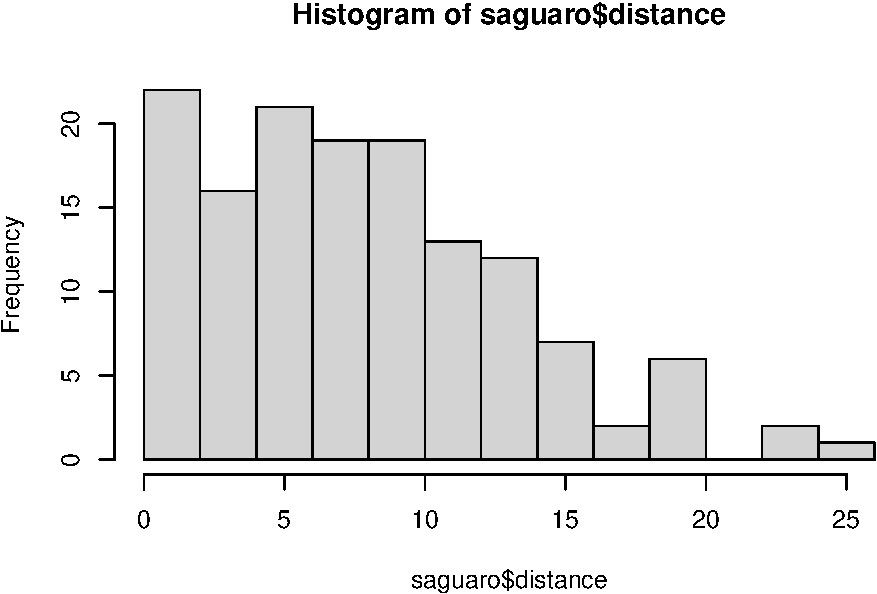
\includegraphics{Module5_Assignment1_AnswerKey_files/figure-latex/unnamed-chunk-4-1.pdf}

\begin{enumerate}
\def\labelenumi{\arabic{enumi}.}
\setcounter{enumi}{4}
\tightlist
\item
\end{enumerate}

\begin{verbatim}
## [1]  0  4  8 12 16 20
\end{verbatim}

\begin{enumerate}
\def\labelenumi{\arabic{enumi}.}
\setcounter{enumi}{5}
\tightlist
\item
\end{enumerate}

\begin{verbatim}
## Warning in formatDistData(saguaro, distCol = "distance", transectNameCol =
## "group", : The transects were converted to a factor
\end{verbatim}

\begin{verbatim}
## # A tibble: 10 x 5
##    `[0,4]` `(4,8]` `(8,12]` `(12,16]` `(16,20]`
##      <dbl>   <dbl>    <dbl>     <dbl>     <dbl>
##  1       5       7        1         0         0
##  2       7       4        4         4         1
##  3       3       4        2         0         3
##  4       5       8        9         4         0
##  5       4       3        2         1         1
##  6       1       1        4         0         0
##  7       2       2        3         3         0
##  8       2       2        2         0         0
##  9       3       3        4         2         1
## 10       6       6        1         5         2
\end{verbatim}

\begin{enumerate}
\def\labelenumi{\arabic{enumi}.}
\setcounter{enumi}{6}
\tightlist
\item
\end{enumerate}

\begin{verbatim}
## Data frame representation of unmarkedFrame object.
##                y.1 y.2 y.3 y.4 y.5
## AB, JA, SK       5   7   1   0   0
## AB, SS, ML       7   4   4   4   1
## CB, CC, MZ       3   4   2   0   3
## EF, LB, YX       5   8   9   4   0
## HA, JB, BD, VM   4   3   2   1   1
## HB, SI, BM       1   1   4   0   0
## JG, AV, MN       2   2   3   3   0
## KH, NT, BS       2   2   2   0   0
## KT, MRD, BC      3   3   4   2   1
## NL, MS, MM       6   6   1   5   2
\end{verbatim}

\begin{enumerate}
\def\labelenumi{\arabic{enumi}.}
\setcounter{enumi}{7}
\tightlist
\item
\end{enumerate}

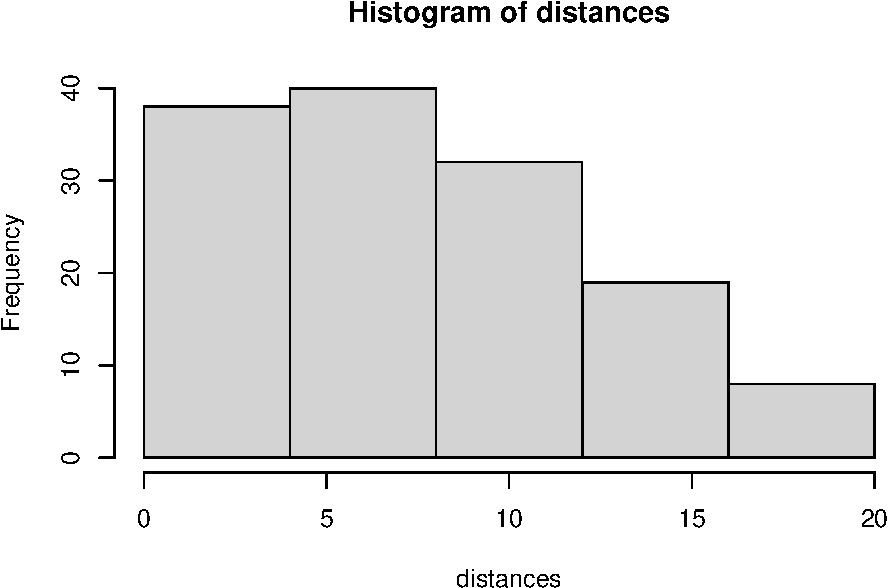
\includegraphics{Module5_Assignment1_AnswerKey_files/figure-latex/unnamed-chunk-9-1.pdf}

\begin{enumerate}
\def\labelenumi{\arabic{enumi}.}
\setcounter{enumi}{9}
\tightlist
\item
\end{enumerate}

\begin{verbatim}
##             nPars    AIC delta   AICwt cumltvWt
## Half Normal     2 213.10  0.00 5.3e-01     0.53
## Hazard Rate     3 213.37  0.27 4.7e-01     1.00
## Exponential     2 230.34 17.24 9.6e-05     1.00
## Uniform         1 242.62 29.53 2.1e-07     1.00
\end{verbatim}

\begin{enumerate}
\def\labelenumi{\arabic{enumi}.}
\setcounter{enumi}{11}
\tightlist
\item
\end{enumerate}

\begin{verbatim}
## Backtransformed linear combination(s) of Density estimate(s)
## 
##  Estimate   SE LinComb (Intercept)
##      49.5 5.66     3.9           1
## 
## Transformation: exp
\end{verbatim}

\begin{enumerate}
\def\labelenumi{\arabic{enumi}.}
\setcounter{enumi}{12}
\tightlist
\item
\end{enumerate}

\begin{verbatim}
##             0.025    0.975
## lam(Int) 39.57627 61.96885
\end{verbatim}

\begin{enumerate}
\def\labelenumi{\arabic{enumi}.}
\setcounter{enumi}{14}
\tightlist
\item
\end{enumerate}

\begin{verbatim}
## # A tibble: 338 x 4
##        X group      length distance
##    <int> <chr>       <dbl>    <dbl>
##  1     1 JG, AV, MN     64       19
##  2     2 JG, AV, MN     64       16
##  3     3 JG, AV, MN     64        0
##  4     4 JG, AV, MN     64        3
##  5     5 JG, AV, MN     64       18
##  6     6 JG, AV, MN     64        0
##  7     7 JG, AV, MN     64       13
##  8     8 JG, AV, MN     64       12
##  9     9 JG, AV, MN     64        0
## 10    10 JG, AV, MN     64        9
## # ... with 328 more rows
\end{verbatim}

\begin{enumerate}
\def\labelenumi{\arabic{enumi}.}
\setcounter{enumi}{15}
\tightlist
\item
\end{enumerate}

\begin{verbatim}
## # A tibble: 10 x 2
##    group          length
##    <chr>           <dbl>
##  1 AB JA SK        164  
##  2 AB, SS, ML      178. 
##  3 CB, CC, MZ      136. 
##  4 EF, LB, YX       59  
##  5 HA, JB, BD, VM  113. 
##  6 HB, SI, BM       48  
##  7 JG, AV, MN       64  
##  8 KH, NT, BS      126. 
##  9 KT, MRD, BC      80.2
## 10 NL, MS, MM      155
\end{verbatim}

\begin{enumerate}
\def\labelenumi{\arabic{enumi}.}
\setcounter{enumi}{16}
\tightlist
\item
\end{enumerate}

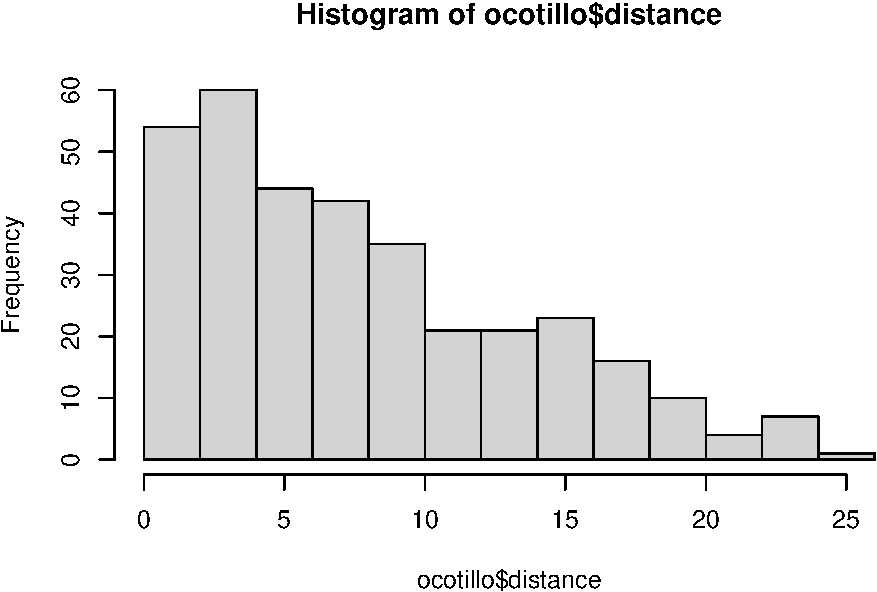
\includegraphics{Module5_Assignment1_AnswerKey_files/figure-latex/unnamed-chunk-16-1.pdf}

\begin{enumerate}
\def\labelenumi{\arabic{enumi}.}
\setcounter{enumi}{17}
\tightlist
\item
\end{enumerate}

\begin{verbatim}
## [1]  0  5 10 15 20 25
\end{verbatim}

\begin{enumerate}
\def\labelenumi{\arabic{enumi}.}
\setcounter{enumi}{18}
\tightlist
\item
\end{enumerate}

\begin{verbatim}
## Warning in formatDistData(ocotillo, distCol = "distance", transectNameCol =
## "group", : The transects were converted to a factor
\end{verbatim}

\begin{verbatim}
## # A tibble: 10 x 5
##    `[0,5]` `(5,10]` `(10,15]` `(15,20]` `(20,25]`
##      <dbl>    <dbl>     <dbl>     <dbl>     <dbl>
##  1      10        8         2         0         0
##  2      17        9         9         7         4
##  3       9       17         8        11         5
##  4       4        8         3         3         0
##  5      22       16         6         6         0
##  6       3        7         5         2         0
##  7      17        6         6         4         0
##  8      13       15         2         0         0
##  9      14        7         2         0         0
## 10      26        7         8         7         3
\end{verbatim}

\begin{enumerate}
\def\labelenumi{\arabic{enumi}.}
\setcounter{enumi}{19}
\tightlist
\item
\end{enumerate}

\begin{verbatim}
## Data frame representation of unmarkedFrame object.
##                y.1 y.2 y.3 y.4 y.5
## AB JA SK        10   8   2   0   0
## AB, SS, ML      17   9   9   7   4
## CB, CC, MZ       9  17   8  11   5
## EF, LB, YX       4   8   3   3   0
## HA, JB, BD, VM  22  16   6   6   0
## HB, SI, BM       3   7   5   2   0
## JG, AV, MN      17   6   6   4   0
## KH, NT, BS      13  15   2   0   0
## KT, MRD, BC     14   7   2   0   0
## NL, MS, MM      26   7   8   7   3
\end{verbatim}

\begin{enumerate}
\def\labelenumi{\arabic{enumi}.}
\setcounter{enumi}{21}
\tightlist
\item
\end{enumerate}

\begin{verbatim}
##             nPars    AIC  delta   AICwt cumltvWt
## Half Normal     2 284.10   0.00 8.0e-01     0.80
## Hazard Rate     3 286.89   2.79 2.0e-01     1.00
## Exponential     2 431.82 147.72 6.7e-33     1.00
## Uniform         1 431.82 147.72 6.7e-33     1.00
\end{verbatim}

\begin{enumerate}
\def\labelenumi{\arabic{enumi}.}
\setcounter{enumi}{22}
\tightlist
\item
\end{enumerate}

\begin{verbatim}
## Backtransformed linear combination(s) of Density estimate(s)
## 
##  Estimate  SE LinComb (Intercept)
##       118 8.3    4.77           1
## 
## Transformation: exp
\end{verbatim}

\begin{verbatim}
##             0.025    0.975
## lam(Int) 103.0058 135.6364
\end{verbatim}

\end{document}
